\documentclass{article}
\usepackage[utf8]{inputenc}
\usepackage{graphicx}   % Para imágenes.
\usepackage{multicol}
\usepackage{amsmath}
\usepackage{dashrule}
\usepackage{geometry}
\usepackage[spanish, mexico]{babel}
\usepackage{subcaption}
\usepackage[svgnames]{xcolor}
\usepackage{tcolorbox}
\usepackage[table,xcdraw]{xcolor}
\usepackage{fancyhdr}
\usepackage{enumitem}
\usepackage{siunitx}
\usepackage[export]{adjustbox}
\usepackage{multirow}

\definecolor{gray(x11gray)}{rgb}{0.75, 0.75, 0.75}
\definecolor{outerspace}{rgb}{0.25, 0.29, 0.3}
\definecolor{pastelgreen}{rgb}{0.47, 0.87, 0.47}
\definecolor{lincolngreen}{rgb}{0.11, 0.35, 0.02}

\geometry{
    a4paper,
    tmargin = 1.7 cm,
    bmargin = 1.7cm,
    lmargin = 1.5cm,
    rmargin = 1.5cm
}



\pagestyle{fancy}
\fancyhf{}
\cfoot{ \thepage  \hspace{0.5pt}\hspace{0.5pt}}
\lhead{Tarea Examen}

\begin{document}

\thispagestyle{plain}


\hrule
\begin{center}
    {\Large \textbf{INSTITUTO NACIONAL DE CANCEROLOGÍA}}
    \vspace{10pt}

    {\Large{{Taller de planeación I}}}
    
    
    \vspace{10pt}

    \hrule

    \vspace{20pt}


    {\Huge \textbf{Guía de tecnicas de planeación}}\\
\end{center}

\hdashrule{\linewidth}{1pt}{1mm}

\begin{flushright}
    {\small Medel Garduño Diego} 
\end{flushright}



\begin{tcolorbox}[colback= pastelgreen, colframe= lincolngreen, title={Consideraciones iniciales}, center title]
    
    Las tecnicas que descritas a continuación comparten una serie de pasos inciales, que toman en cuenta desde la entrada al sistema de eclipse hasta como colocar un campo de tratamiento y su respectivo MLC (Cabe resaltar que la tecnica de IMRT no hace uso de colocar un MLC).

    \vspace{10pt}

    \textbf{Pasos iniciales}
    \begin{enumerate}
        \item Entrar a eclipse, haciendo uso de una usuario y contraseña antes provista.
        \item Ir al apartado de planificación de haz externo.
        \item Colocar la identificación del paciente, designada como id.
        \item Una vez encontrado el paciente, se desplegara una pestaña en la cual se deben seleccionar las etapas de tratamiento actuales, en caso de no haber crear una nueva etapa de tratamiento, considerando la colección de imagenes del respectivo paciente.
        \item Al generar una nueva etapa de tratamiento, solo se encontrará las estructuras contorneadas por los medicos y un set de imagenes, obtenidas de un tomografo en los planos sagital, axial y coronal.
        \item Como proximo paso se debe observar cual es la estructura de interes, de manera general el ICRU 83 designa al PTV como el volumen de planeación. 
        \item Se debe revisar que la estructura en tres dimensiones del paciente coincida con \textit{cosmo}, figura que ayuda al planeador a identificar si eclipse y la manera en la que se simulo un paciente es la misma. 
        \item Tambien se debe revisar que el isocentro coincida con los balines puestos al paciente. Este es un metodo utilizado para que la posición de un paciente sea reproducible bajo otras condiciones.
        \item Seguido a lo anterior y practicidad a la hora de aplicar un tratamiento, se debe considerar que las coordenadas del isocentro esten redondeadas a 0 o 0.5 cm
        \item Revisado todo esto se debe ir a la pestaña de \textit{insertar}, que se encuentra en la barra superior de la intefaz de eclipse
        \item Una vez completado el paso anterior, se debe seleccionar la pestaña que dice \textit{nuevo plan}
        \item A este plan se le debe de asignar una identificación, es decir, un nombre, se debe seleccionar sobre que estructura (PTV) va a trabajar, la orientación que considerará para el calculo de dosis, la prescripción de dosis y por ultimo el acelerador lineal donde se efectuará el tratamiento.
        \item Considerando en que parte del cuerpo se encuentre el PTV se debe considerar que energia utilizar, de manera general se considera que:
            \begin{itemize}
                \item Si el PTV esta en cabeza, cuello o es una mama utilizar una energia de 6x
                \item En cambio si el PTV se encuentra en una region del tronco superior (como el torso) o tronco inferior, utilizar una energia de 15x
            \end{itemize} 
        \item Nuevamente en la pestaña de insertar se debe seleccionar \textit{nuevo campo}
        \item En este campo se debe especificar la energía a utilizar y la rotación del gantry y en su defecto del colimador.
        
    \end{enumerate}

\end{tcolorbox}


\begin{tcolorbox}[colback=pastelgreen]

    \begin{enumerate}
        \item[16.] A este nuevo campo se le debe asignar un MLC que debe estar ajustado al PTV dejando un margen de 0.5 cm
    \end{enumerate}
    
\end{tcolorbox}



\section{Tecnica conformal AP PA}


\subsection{Descripción}

Esta tecnica considera la indicencia de dos campos, uno que entre de forma anterior y sale por la parte posterior y otro que entra por la parte posterior y sale por la parte anterior, de ahi que su nombre sea tecnica antero posterior, postero anterior. 

\vspace{10pt}

\subsection{Establecimiento de la angulación del gantry y determinación del peso de los campos}

Para el haz AP se debe colocar el gantry a 0 grados, mientras que para el PA el gantry debe estar a 180 grados.Una vez que se han generado dos campos con dichas angulaciones, se deben ajustar los MLC tal y como se especifico en los pasos inciales. Dado esto el planeador debe pedirle a eclipse que haga el calculo de dosis, cuando lo haya acabado es importante seleccionar que cada campo debe tener un peso tal que su suma sea del 100 porciento. 

\vspace{10pt}

\subsection{Consideraciones especiales: punto caliente}

Cuando se hayan ajustado que cada campo contribuye con un 50 porciento del peso total, de debe corroborar que la distribución de dosis cubra de manera adeacuada el PTV, y que el punto caliente de cada corte no este en algun organo de riesgo. Esta tecnica se utiliza de forma frecuente para tratamientos paliativos de hueso, como por ejemplo la columna, dada su posición en la mayoria de casos se debe cuidar que el punto caliente no se encuentre en los intestinos. Si los puntos calientes estan muy arriba o muy abajo del PTV se deben modificar los pesos de los campos, de tal manera que uno contribuya con más peso que el otro, de esta manera se manipula la posición de los puntos calientes. Este proceso puede ayudar tambien a bajar la dosis del punto de dosis maxima.

\vspace{10pt}

\subsection{Proceso de normalización}

Al termino de este proceso, y considerando el rango en el que se encuentra la dosis, se debe hacer una normalización, es decir, si la prescripción del tratamiento es de 800 cGy y la interfaz de ecilpse indica que existe un punto al que se le estan dando más de 800 cGy de dosis, este punto ahora será el que entrega el 100 porciento. Una vez normalizado el plan, se debe elegir una curva con la cual se cubra el mayor porcentaje de PTV, sin que el punto de dosis maxima sobrepase el 15 porciento por encima de la dosis de prescripción. De manera clinica se acepta como adecuada hasta la curva del 88 porciento, la del 85 tambien se puede aceptar, sin embargo esta implica hacer una revisión más extenuante para designar si el aplicar esa curva no presenta un riesgo toxico para el paciente. 

\subsection{Ejemplo practico}

\begin{figure}[h!]
    \centering
    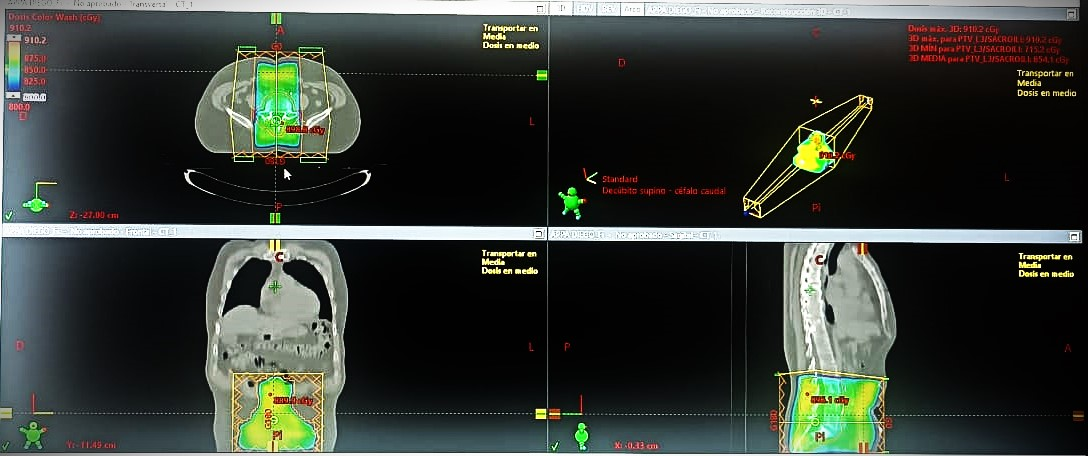
\includegraphics[scale = 0.4]{appa.jpg}
    \caption{Ejemplo de un plan realizado con una tenica de AP PA}
    \label{a1}
\end{figure}





En la figura \ref{a1} se presenta un ejemplo de esta tecnica y se muestra un poco de como es la interfaz grafica de eclipse. Se trato un hueso que forma parte de las vertebras lumbares, se observa como hay dos campos opuestos, uno que entra de manera anterior y otro posterior. Este plan tuvo una cobertura del 99 porciento y el punto de dosis maxima se elevo un 13 porciento de la dosis de prescripción, lo cual aun entra en el rango de lo aceptable.

\section{Tecnica corformal AP PA con oblicuos}


\subsection{Descripción}

Esta tecnica es similar a la anterior, solamente que ahora se agregan dos campos, los angulos en los que entran pueden variar, sin embargo de manera habitual se considera 150 y 210 grados. 

\vspace{10pt}

\subsection{Diferencia entre una tecnica AP PA normal y una que utiliza oblicuos}


Para este caso se va a segur la misma secuencia de pasos, por tanto cuando ya se tengan los campos AP y PA con sus respectivos MLC, se deben añadir dos más, uno de ellos debe tener una rotación de gantry a 150 grados y el otro a 210 grados, de esta forma se generan dos haces que entran de forma oblicua al volumen de planeación (PTV). 

\vspace{10pt}


Despues de agregar las MLC y haberlas ajustado al PTV, se le debe pedir a eclipse que haga el calculo de dosis. Cuando este proceso termine, se debe designar que el peso de los campos sea del 100 porciento, es decir, de manera inicial cada campo debe contribuir con un 25 porciento del peso total. Sin embargo, es importante tomar en cuenta que los campos no deben tener pesos similares, se recomienda que el peso de los campos oblicuos sea del 15 porciento, para que así los campos AP y PA tengan mayor peso.

\subsection{Uso de subcampos y dosis maxima}

Es importante esclarecer que el uso de subcampos es algo que depende de la distribución de dosis, es decir, se recomienda para este tipo de tecnicas que la distribución sea lo más uniforme que se pueda, lo cual implica que hay eliminar aquellas zonas que muestren un alto gradiente, respecto a los demas gradientes. Entonces si existen zonas de alto gradiente, se recomienda hacer uso de subcampos para asi generar un distribución de dosis mas homogenea, de igual forma esto puede contribuir con la disminución de la dosis maxima en un punto. 

\vspace{10pt}


\subsection{Cobertura}


Una vez que la dosis es homogenea ya sea con el uso de subcampos o en dado caso que no los necesite, es importante observar la cobertura. Algunos reportes ICRU relatan que se considera una buena cobertura si esta es mayor al 95 porciento del PTV. Sin embargo, la cobertura estará influencia a otros criterios, entre ellos los clinicos, es decir, que tanto el medico indica que debe cubrir, en dado caso la cobertura esta sujeta aun criterio mas especializado. 

\vspace{10pt}


Por tanto es importante que cubra el mayor porcentaje de PTV, sin que el punto de dosis maxima sobrepase el 15 porciento, por arriba de este umbral, se debe evaluar si el tratamiento puede darse y no es demasiado toxico para el paciente.

\vspace{10pt}



\subsection{Ejemplo practico}

\begin{figure}[h!]
    \centering
    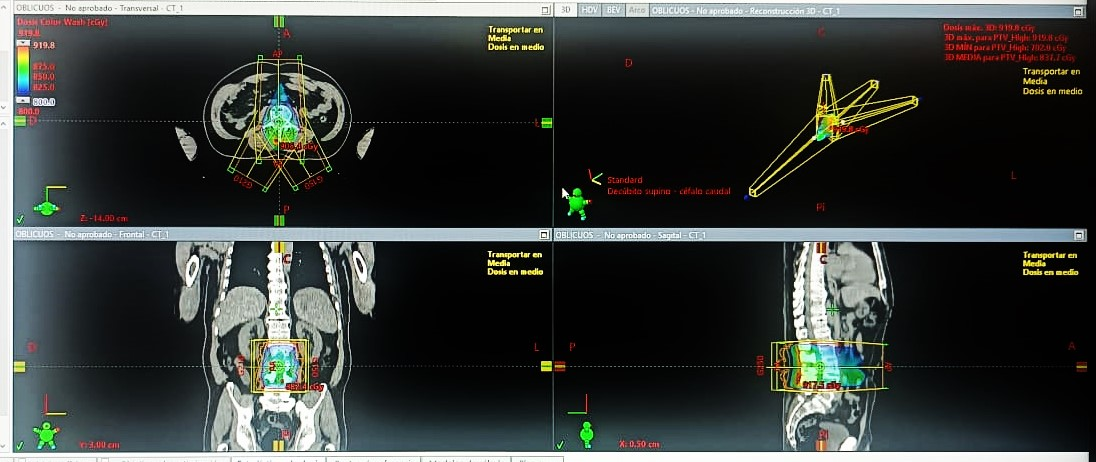
\includegraphics[scale = 0.4]{oblicuos.jpg}
    \caption{Ejemplo de un plan realizado con una tenica de campos oblicuos}
    \label{a2}
\end{figure}


En este caso la figura \ref{a2} muestra como deben ser los campos cuando se utiliza una tecnica de campos oblicuos, de igual manera se ilustra que la distribución de dosis opta una figura en forma de un especie de huevo, lo cual sirve para disminuir el volumen de tejido irradiado, que en consecuencia implica una mejor protección a los organos de riesgo. 

\vspace{10pt}

Algo a mencionar de este plan es que su cobertura fue del 93 porciento y la dosis maxima tuvo un mayor valor que en la tecnica de AP PA, sin embargo estos valores no son suficientes para evaluar si una tecnica es mayor que otra, cada una tiene sus diferencias y ventajas respecto a lo que se busca tratar. La diferencia entre los oblicuos y el AP PA, tambien puede deberse a la dificultad de la tecnica, mientras que hacer un plan con AP PA es relativamente sencillo, los oblicuos implican una mayor destreza. 


\section{Holocraneo}

\subsection{Descripción}

Esta tecnica esta definida para tratar pacientes con alguna afección a nivel de cerebro, es un tratamiento paliativo y se busca que sea lo menos toxico posible para la persona irradiada, para ello es importante tener control sobre el punto de dosis maxima y la homogeneidad de la distribución de dosis. Un punto a recalcar es que de manera general se utiliza una prescripcion de 30 en 10, es decir, se aplican 30 Gy en un total de 10 sesiones.

\subsection{Sobre la planeación}

Cuando se realiza un holocraneo es importante tomar en cuenta que se hará uso de dos campos como en una tecnica AP PA, sin embargo, la angulación es distinta, para esta tecnica se busca que la dosis entre de manera temporo parietal, entonces se coloca el grantry a 90 y 270 grados para cada campo. Una vez colocados los campos es importante observar la distribución de dosis, debe ser homogenea, es decir, en particular no deben verse zonas con mayor gradiente que otras, tomando como punto de referencia la linea sagital que divide al cuerpo.

\subsection{Inhomogenidades en la distribución}

En dado caso que exista un desbalance en la distribución de dosis, esta puede deberse a que en la simulación la cabeza del paciente tenia cierta angulación respecto al plano que pasa por su eje sagital. Para solucionar este percanse se debe hacer una modificación en los pesos de los campos, de tal forma que el campo que presenta un mayor gradiente de dosis tenga menor peso que aquel que tuvo menor gradiente.

\subsection{Organos de riesgo}

Un punto importante en esta tecnica es la protección de los organos de riesgo, como lo es el cristalino, ya que la prescripción demanda una cantidad que si da de lleno en el cristalino puede generar opacidad o en cierto caso ceguera temporal. Es por ello que es importante mantener la dosis maxima de los cristalinos por debajo de los 10 Gy, para se debe colocar las hojas del MLC principal cubriendo estas estructuras, para asi darles una protección adecuada. Si esto si hiciera con un subcampo, la protección buscada solo se lograría aumentando mucho los pesos de los subcampos, lo cual tendria como resultado huecos en la distribución de dosis.

\vspace{10pt}


Una consecuencia de la protección de los cristalinos es que la cobertura se puede ver afectada, por tanto, este proceso tambien queda a elección del medico, si elige que es más importante que la dosis cubra el mayor porcentaje del PTV o prioriza los organos de riesgo.


\subsection{Ejemplo practico}

\begin{figure}[h!]
    \centering
    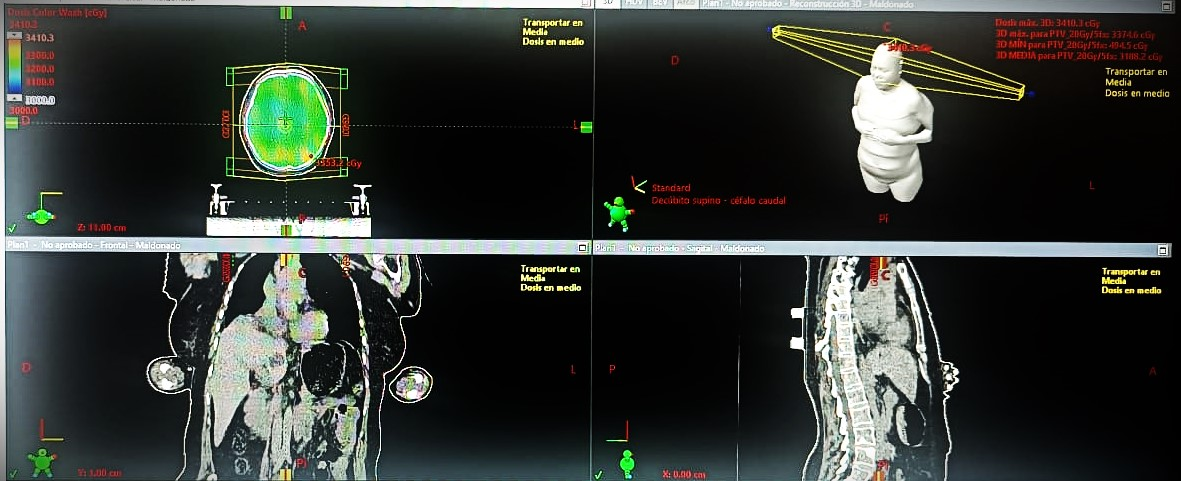
\includegraphics[scale = 0.4]{holo.jpg}
    \caption{Ejemplo de un plan realizado con una tenica de holocraneo}
    \label{a3}
\end{figure}


En la figura \ref{a3} se ilustra como se efectua una tecnica de holocraneo, en la imagen superior derecha se muestra de manera clara como deben de entrar los campos en el paciente, en la figura superior izquierda se logra observar que la dosis es homogenea y no se encuentra cargada para ningun lado. En este plan se puso como objetivo proteger a los cristalinos, es por ello que la dosis maxima que recibe cada uno quedo al rededor de los 3 Gy, lo cual puede considerarse como aceptable. La cobertura no se vio afectada del todo, sin protección en los cristalinos a una curva del 88 porciento, se lograba una cobertura del 98.6 porciento, mientras que cubriendo a los cristalinos a la misma curva la cobertura disminuia al 98.04 porciento. 


\newpage

\section{Tecnica conformal de caja}

\subsection{Descripción}


Esta tecnica es paliativa, normalmente utilizada en PTV que tengan una geometria similar a la de un rectangulo en 2D y una caja en 3D, es por ello que la tecnica lleva este nombre. Consiste en el uso de cuatro campos, cada uno separado del otro en 90 grados.


\subsection{Sobre la tecnica}


En principio de debe seguir la misma serie de pasos que en un AP PA, solamente que se deben agregar dos campos más, uno a 90 grados y el otro a 270 grados. Una vez creados, se les debe asignar un MLC, ajustado al PTV, despues indicarle a eclipse que haga el calculo de dosis, cuando temine se debe designar que la suma de los pesos de los campos sea del 100 porciento, para esta tecnica tambien es importante considerar la homogeneidad de la distribución de dosis, por lo que se deben modificar los pesos de los campos hasta que la dosis sea lo más homogenea posible.

\vspace{10pt}

Es importante mencionar que al igual que en las otras tecnicas debe de haber un control en el punto de maxima dosis, este no debe de exceder el 15 porciento. Un aspecto caracteristico de esta tecnica es que los puntos de dosis elevada se van a encontrar en alguna de las aristas de las caja.


\subsection{Consideraciones finales}


De igual forma se busca que la cobertura del PTV sea lo más cercana a 100 porciento que se pueda, es importante explicar que en este tipo de tecnica el volumen irradiado será mayor que el volumen del PTV. 

\subsection{Ejemplo practico}

\begin{figure}[h!]
    \centering
    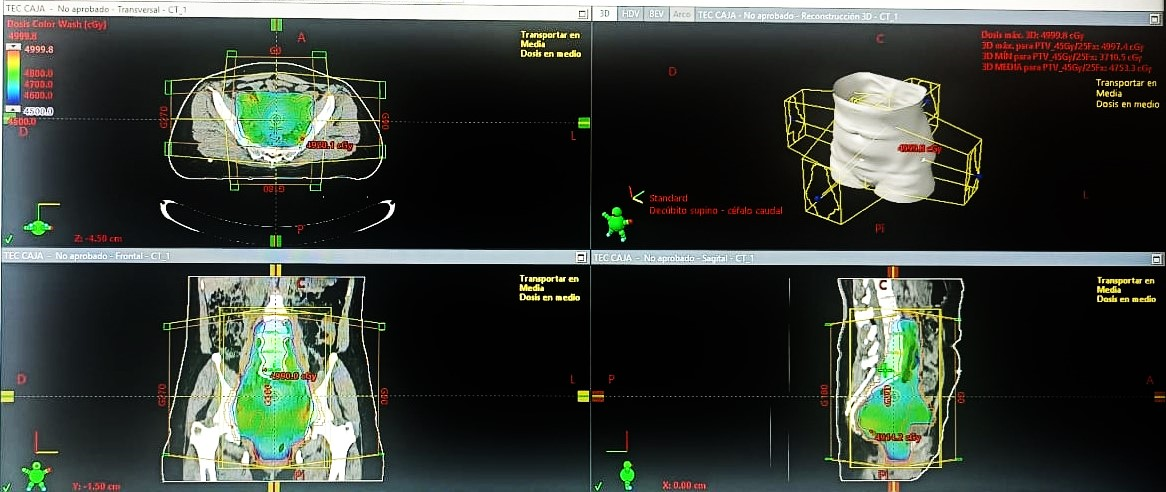
\includegraphics[scale = 0.4]{caja.jpg}
    \caption{Ejemplo de un plan realizado con una tenica de caja}
    \label{a4}
\end{figure}


En este ejemplo se hizo un plan para tratar una vertebra de forma paliativa, por lo que se dieron 4500 cGy en 25 fracciones. Se conformo el PTV de tal forma que se cubrio 98 porciento del volumen, sin embargo como el PTV no tiene una geometria exactamente igual a la de una caja, el volumen irradiado es mayor al volumen del PTV.


\section{Tecnica IMRT}

\subsection{Descripción}

Esta tecnica se describio en el reporte del ICRU 83, donde se establecieron algunas definiciones que resultan distintas a las utilizadas para las tecnicas conformales presentadas anteriormente. Como primer elemento aqui ya no se busca la uniformidad, ya que habrán zonas que tengan un gradiente mayor de dosis y esto es debido en principio a la naturaleza de la tecnica que se basa en la diferencia de las fluencias entre los campos. Es preciso especificar que esta tecnica es realizada por el sistema de planeación, a partir de iteraciones, donde busca la fluencia adeacuada considerando un parametros dados por el planeador.

\subsection{Sobre la tecnica}

En principio se deben establecer entre 7 y 9 campos, repartidos de manera simetrica, es decir, que entre cada campo haya la misma angulación. En este caso no hay que introducir MLC, el mismo optimizador de eclipse se encargara de establecer los MLC y ajustar las hojas de la manera que considere mejor. Para tener un buen resultado hay que introducir al optimizador dos valores, uno de ellos que represente la dosis para el 95 porciento del PTV, y ese será el minimo, por otra parte segundo valor esta dado por la dosis maxima al 110 porciento.

\vspace{10pt}

Con estos valores el programa buscara optimizar cual es la configuración adecuada de hojas del MLC para llegar a ese resultado. Cuando haya llegado al objetivo, mostrara los campos y los MLC, como paso final se debe revisar que la dosis cubra bien el PTV y que no falte en ninguno de los cortes de la tomografia.

\section{Ejemplo practico}


\begin{figure}[h!]
    \centering
    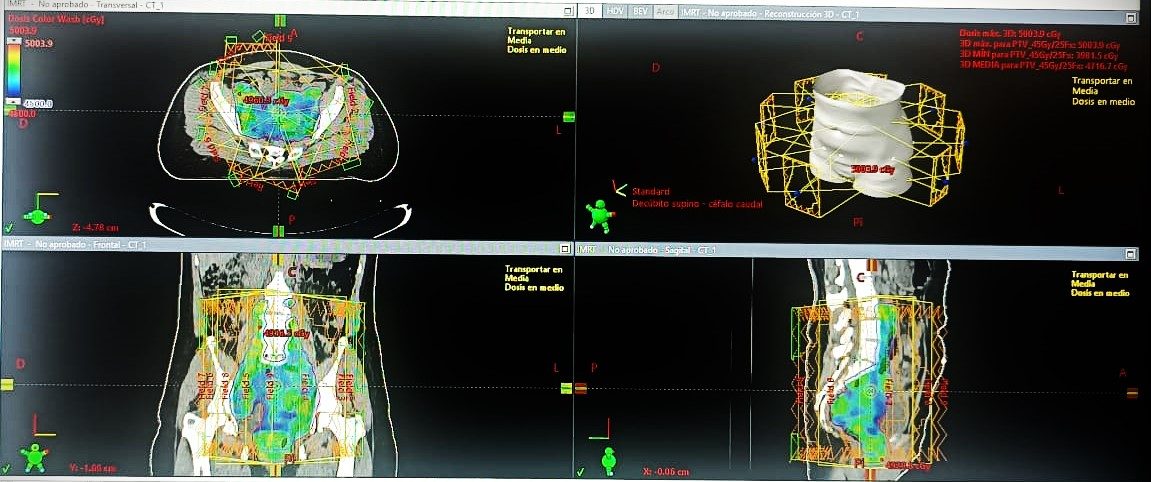
\includegraphics[scale = 0.4]{IMRT.jpg}
    \caption{Ejemplo de un plan realizado con una tenica de IMRT}
    \label{a5}
\end{figure}



En la figura \ref{a5} se muestra la tecnica de IMRT, donde se consideraron 7 campos, cada uno de ellos separado en 40 grados. Se utilizo el mismo paciente que en la tecnica de caja, esto para comparar las diferencias entre cada tecnica. La principal diferencia es el volumen irradiado, que es muy similar al volumen del PTV, considerando el indice de conformidad (valor que indica el grado en el que el volumen irradiado y el volumen del PTV son similares), que fue de 1.11 para IMRT y para la tecnica de caja fue de 1.56, en este sentido se modulo mucho mejor la forma del PTV, cuidando asi la irradiación a tejido sano. 








\end{document}